\subsection{Calibrating a new gyrochronology relation}
\label{sec:calibration}

To calibrate a new gyrochronology relation we fit an empirical power-law
relation, augmented with a Gaussian process, to a grid of kinematic ages and
open cluster stars.
These cluster stars have precise rotation periods measured from Kepler and K2
light curves, and well-determined ages from cluster-based isochrone fitting.
In this section we describe how we fit our model to these data.

\subsubsection{The model}

To calibrate a new empirical gyrochronology relation
we used a composite model, consisting of an underlying mean function,
augmented with a Gaussian process.
The mean function is similar to previous empirical gyrochronology models and
consists of two separable power-law relations: one describing the relationship
between rotation period and age, and the other between rotation period and
color \citep[\eg][]{barnes2003, barnes2007, mamajek2008, meibom2015, angus2015,
angus2019}.

Our mean function is comprised of a single power-law in age, $f(t)$, and a
broken power law in color, $g(C)$:
\begin{equation}
P_\mathrm{rot} = f(t) + g(C),
\end{equation}
where $P_\mathrm{rot}$ is rotation period in days, $t$ is age in Gyr, and C is
Gaia color: $\mathrm{G_{BP} - G_{RP}}$.
The age power-law is defined as,
\begin{equation}
f(t) = at^n,
\end{equation}
following the functional form first described in \citep{barnes2003}, where $a$
and $n$ are free parameters.
The broken power-law in color is defined as,
\begin{equation}
g(C) = \delta
\left(\frac{m_1}{1 + e^{s \delta}}\right)
+ \left(\frac{m_2}{1 + e^{-s \delta}}\right),
\end{equation}
where $s$ is a parameter that determines how smooth the break is, $m_1$ is the
slope below (bluewards of) the power-law break, $m_2$ is the slope above
(redwards of) the break, and
\begin{equation}
\delta = C - C_\mathrm{break},
\end{equation}
where $C_\mathrm{break}$ is the color of the power-law break.
In this model, $s$, $m_1$, $m_2$, and $C_\mathrm{break}$ were all free
parameters.

A Gaussian process model then distorts this mean model to provide a better fit
to the data.
In other words, it models the residuals between the mean model and the data.
We used a simple squared exponential kernel function which has only two free
parameters, an amplitude, $A$ and a length scale, $l$.
This kernel function is defined as,
\begin{equation}
k_{ij} = A \exp\left[{\frac{-(x_i - x_j)^2}{2l^2}}\right]
\end{equation}

The parameters were optimized using the {\tt exoplanet} code \citep{exoplanet}.
% The posterior PDFs of these parameters of the power-law relations, and the
% hyper-parameters of the GP kernel were explored with MCMC.
% We used the {\tt exoplanet} \citep{exoplanet} and {\tt PyMC3} \citep{pymc3}
% Python packages to fit this model to the data.

\subsubsection{Formatting the data}

A Gaussian process is only an appropriate model for data generated by a
Gaussian process.
Data with large numbers of outliers or with inaccurately estimated
uncertainties are not Gaussian-distributed and therefore cannot be described
with a Gaussian process.
Rotation period measurements are rarely generated by a Gaussian process for
two main reasons.
Firstly, the uncertainties on rotation period measurements can rarely be
described as Gaussian because they are often plagued by harmonics/aliases and
spurious measurements.
Secondly, the relationship between rotation period and color often has a large
amount of intrinsic scatter.
The is especially true for young stars and M dwarfs, where there is little
correlation between rotation period and age.
This scatter is not generated purely by measurement uncertainties which means
that it is not well-described by a Gaussian process.
This non-Gaussian nature of rotational data necessitated a certain amount of
data formatting or `massaging' in order to fit our model to the data.
We acknowledge that some of the choices we make during this stage are somewhat
arbitrary, and other choices may have worked equally well.
However, in the end our goal was to produce a gyrochronology model that is
reasonably representative of the data.

There are three main approaches we took:
\begin{itemize}
\item {\bf Trimming the cluster data}.
We used a number of open clusters to calibrate our model: Praesepe, the
Hyades, NGC 6811, NGC 6819, and Ruprecht 147.
Although the rotation periods of most G and K stars in these clusters fall on
a tight sequence, Praesepe contains a number of M dwarfs with measured periods
that are highly stochastic.
Given that the scatter in M dwarf rotation periods is intrinsic: it is not
produced by measurement uncertainties, these data are not well-described by a
Gaussian process.
For this reason, we removed M dwarfs with stochastic rotation periods from our
calibration sample.
We removed all cluster stars with rotation periods shorter than one day and
\gcolor\ $>$ 2.2.
We also removed cluster stars with {\it both} \prot\ $<$ 11 days {\it and}
\gcolor\ $>$ 1.5.
Although the Pleiades cluster contains a number of stars with measured
rotation periods, it is too young to have enough members that have converged
onto a tight rotation sequence so we were unable to include it in our
calibration sample in this work.
\racomment{Will probably need to include Pleiades at some point!}

\item {\bf Applying cuts to the kinematic data.}
As with the cluster data, the kinematic data also needed to be Gaussian
distributed.
For this reason, we removed stars whose rotation periods are not
determined by their age and color.
This includes subgiants, young stars, and binaries.
Subgiants were cut by removing stars with Gaia $M_G$ absolute magnitude less
than 4 \racomment{check this}, and stars with {\it both} \gcolor\ $<$ 1.5 {\it
and} kinematic age $>$ 6 Gyr.
Binaries were cut by fitting a 6th order polynomial.... etc.
Here we define `young stars' to mean stars that are too young to have
converged onto the slow rotator sequence.
These stars have rotation periods shorter than the bulk of the rotation period
distribution.
These young stars were removed by calculating their gyro-ages according to the
\citet{angus2019} empirical relation, and then excluding stars with gyro-ages
younger than 0.7 Gyr.
Hot stars...

\item {\bf Converting kinematic data to a grid.}
Even with these cuts, we were not able to get a good fit to the data for two
main reasons.
Firstly, after these cuts we were left with around 20,000 stars which is a)
expensive and b) probably overkill.
Secondly, we were not including age uncertainties in our fit.
For the clusters we can maybe get away with this, but the uncertainties on the
kinematic are non-negligable \citep[likely 1-2 Gyr][]{lu2021}).
To get around this issue, instead of fitting our GP model to the raw data, we
instead converted it to a grid.
\end{itemize}

\begin{figure}
\caption{
}
  \centering 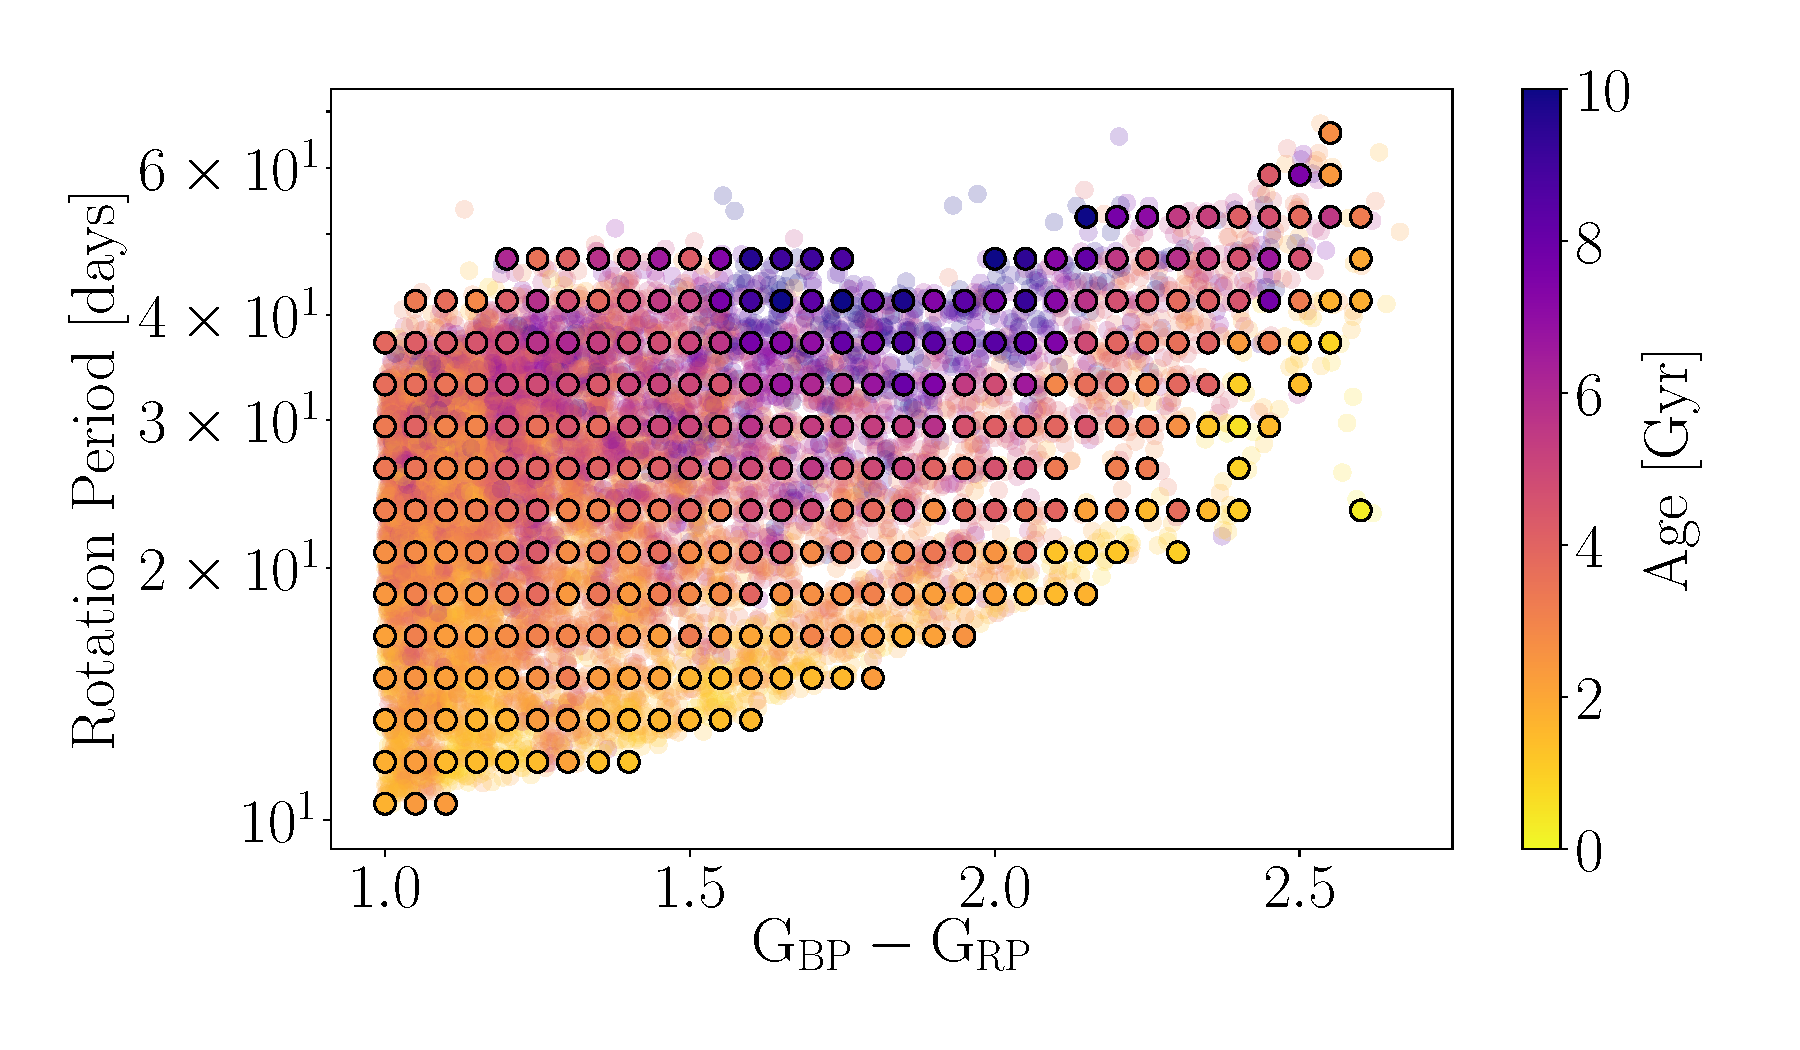
\includegraphics[width=1\textwidth]{grid_points}
\end{figure}

\begin{figure}
\caption{
}
  \centering 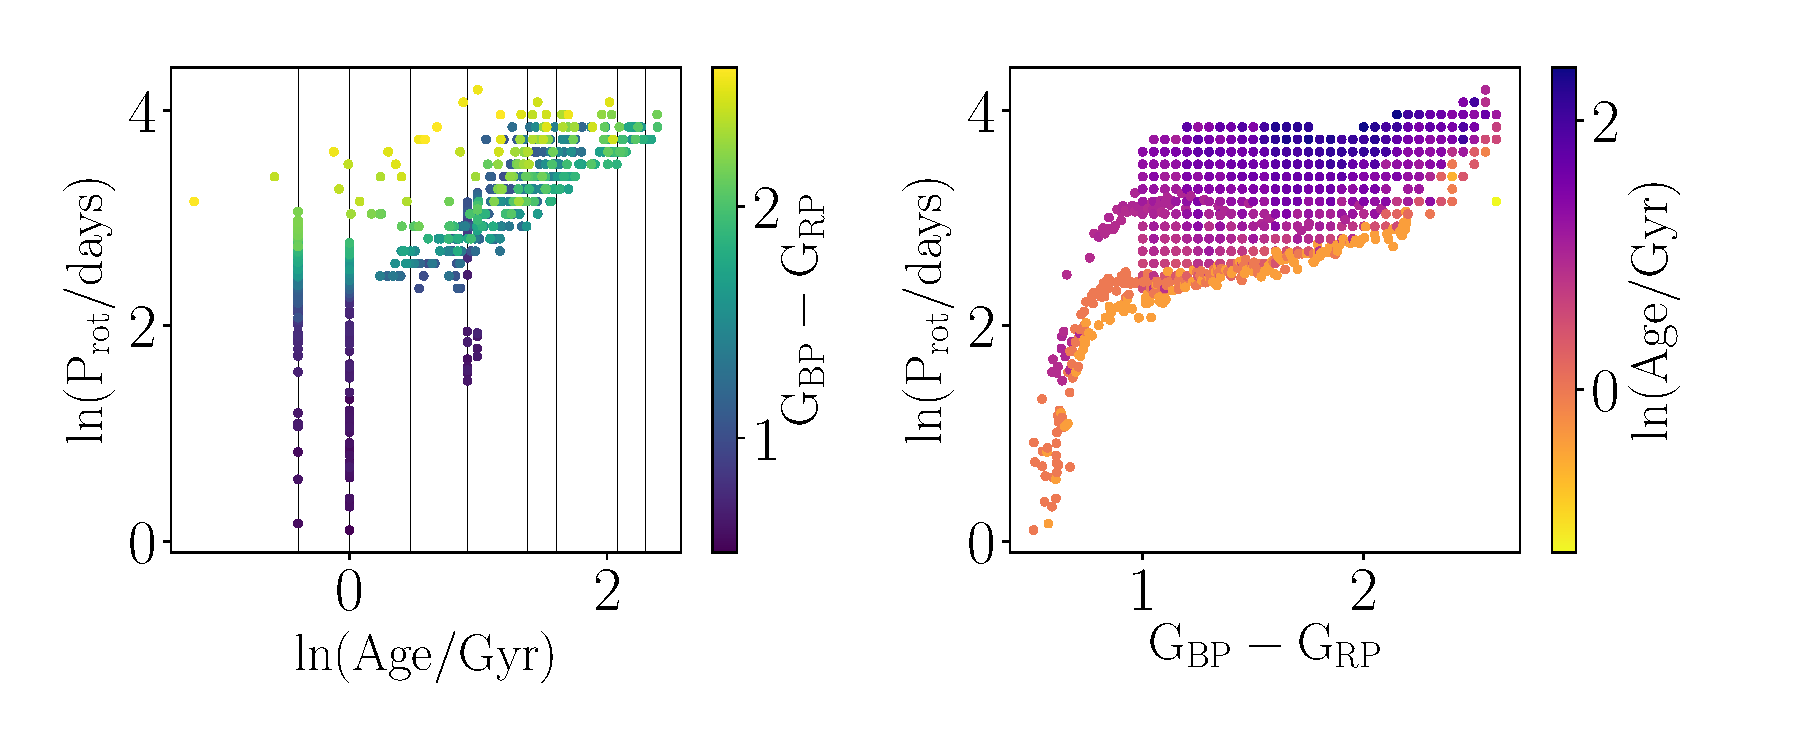
\includegraphics[width=1\textwidth]{gp_fit_data_multi-panel}
\end{figure}

\begin{figure}
\caption{
}
  \centering 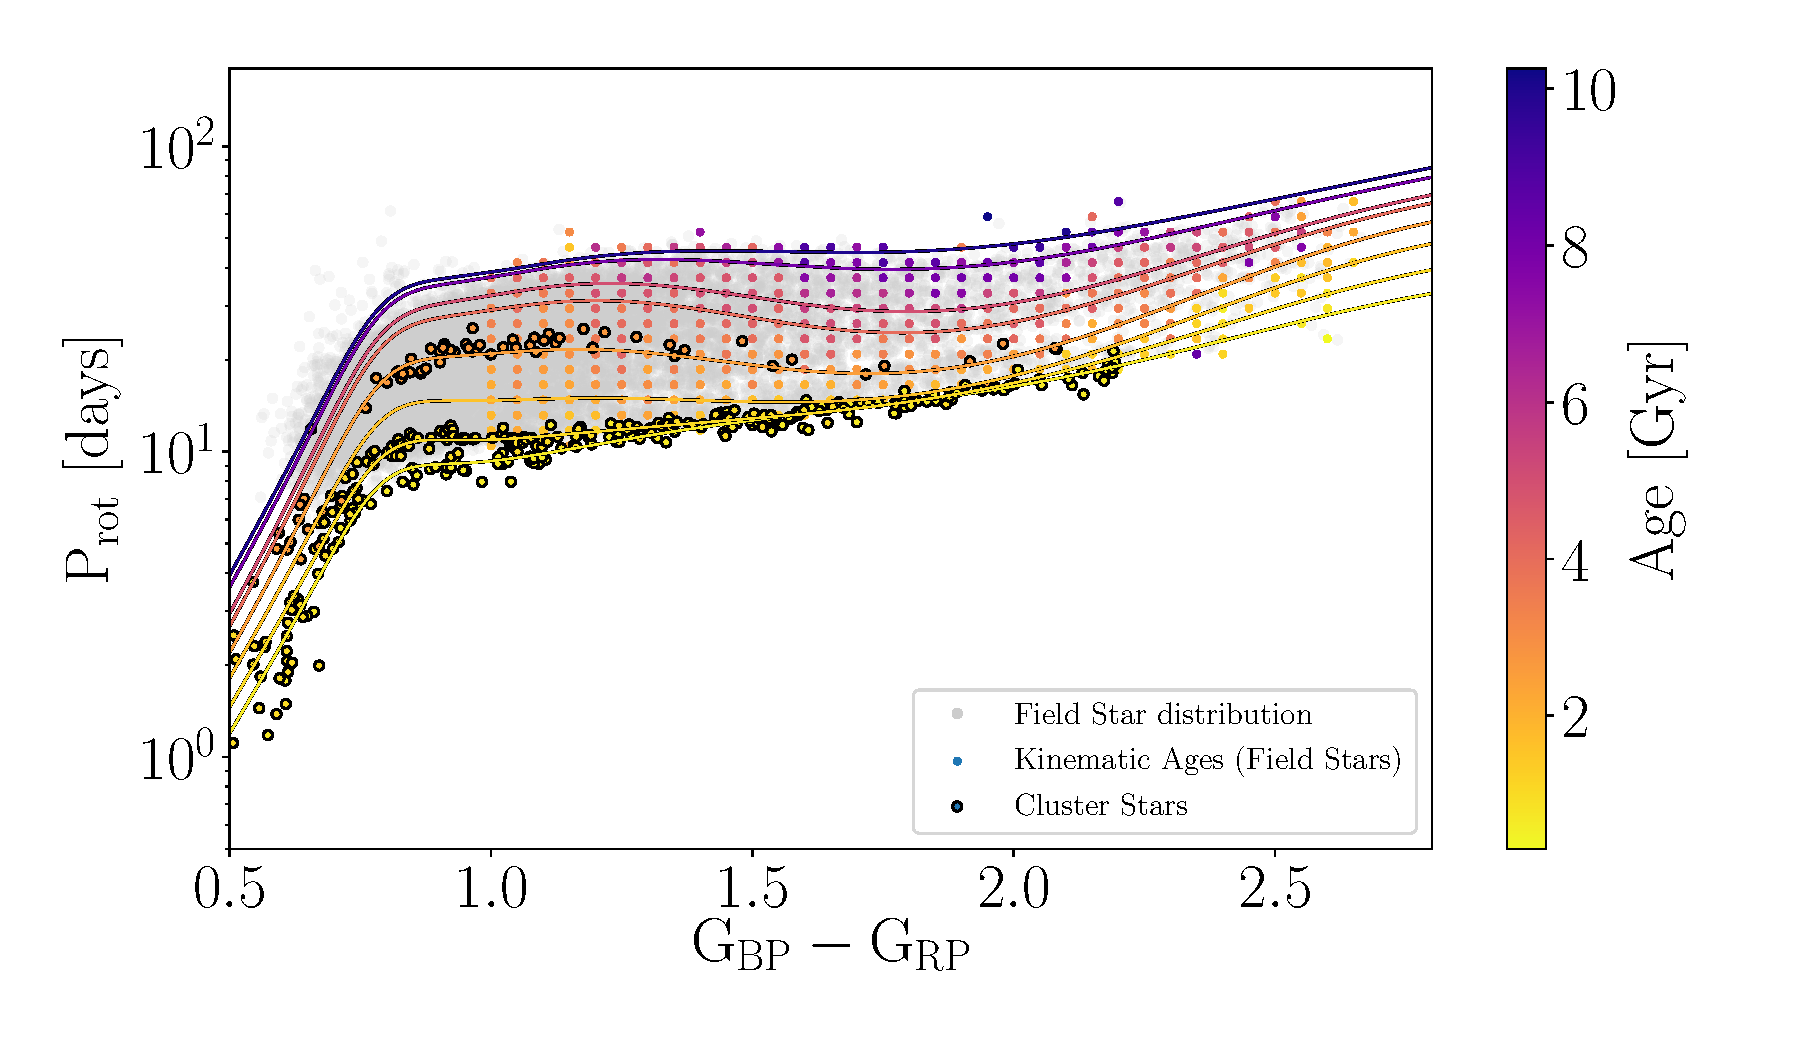
\includegraphics[width=1\textwidth]{gp_fit}
\end{figure}

